\section{Optical Character Recognition}

\begin{frame}{Bearbeitungsschritte}
\begin{columns}
\begin{column}{0.6\textwidth}
\begin{enumerate}
\item {\scriptsize Vergr\"osserung und Graustufen}
\item {\scriptsize Blurring (Bildgl\"attung)}
\begin{enumerate}
\item {\tiny Gaußsche Unsch\"arfe:Effektiv beim Entfernen von Rauschen} 
\item {\tiny Median Unschärfe: Effektiv gegen „Salz- und Pfefferrauschen“ (Flecken)}
\end{enumerate}
\item {\scriptsize Thresholding (Schwellenwertverfahren)}
\begin{enumerate}
\item {\tiny Otsu: w\"ahlt automatisch einen geeigneten Schwellenwert aus}
\item {\tiny Binary-Inv.: Die Werte derart getauscht, dass schwarz zu weiß wird und umgekehrt $\rightarrow$ führt zur besseren Erkennung von Konturen}
\end{enumerate}
\item {\scriptsize Dilation (Morphologische Transformation)}
\begin{itemize}
\item {\tiny Wird auf Binärbildern angewandt und erfordert zwei Eingaben: Originalbild $+$ Strukturierungselement (Kernel)}
\item {\tiny Ein Pixelelement wird 1, wenn ein Pixel im Kernel 1 ist $\rightarrow$ weißer Bereich im Bild wird vergrößert}
\end{itemize}
\end{enumerate}
\end{column}
\begin{column}{0.40\textwidth}
    \begin{center}
        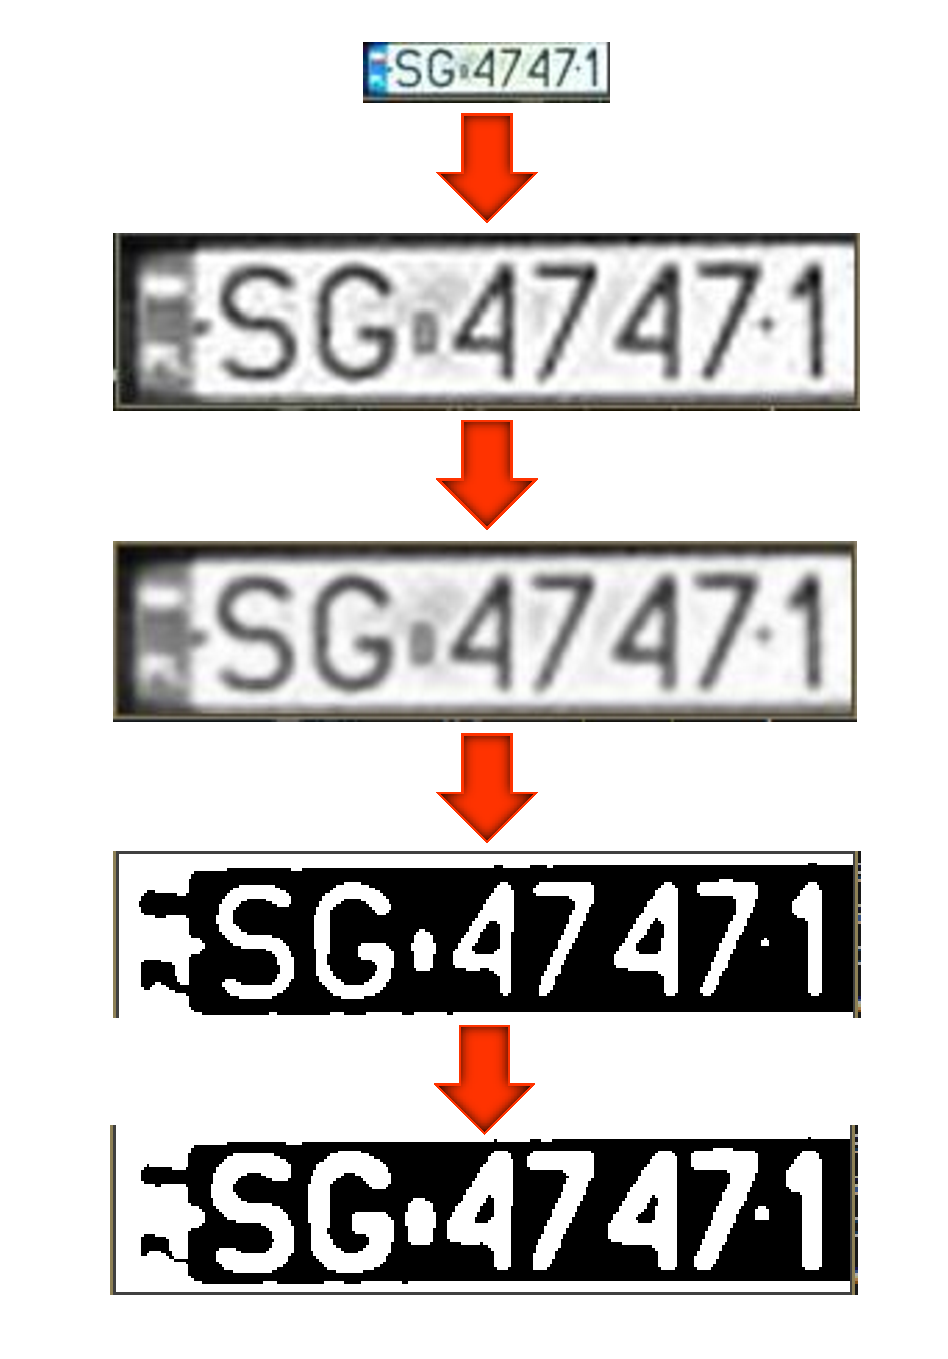
\includegraphics[width=\textwidth]{img/preprocessing}
    \end{center}
\end{column}
\end{columns}
\end{frame}

\begin{frame}{Aussortierung der Konturen}
\begin{itemize}
\item {\textit{\scriptsize Genutzt werden die Werte x,y,w,h (Werte der Kontur) sowie width und height (Breite und Höhe des Bildes)}}
\item {\scriptsize Es werden nur Konturen berücksichtigt, die folgende Bedingungen erf\"ullen:}
\end{itemize}
\begin{eqnarray}
    \frac{height}{h} > 3
    \\
    \frac{h}{w} < 1.2
    \\
    \frac{width}{w} > 50
\end{eqnarray}
    \begin{center}
        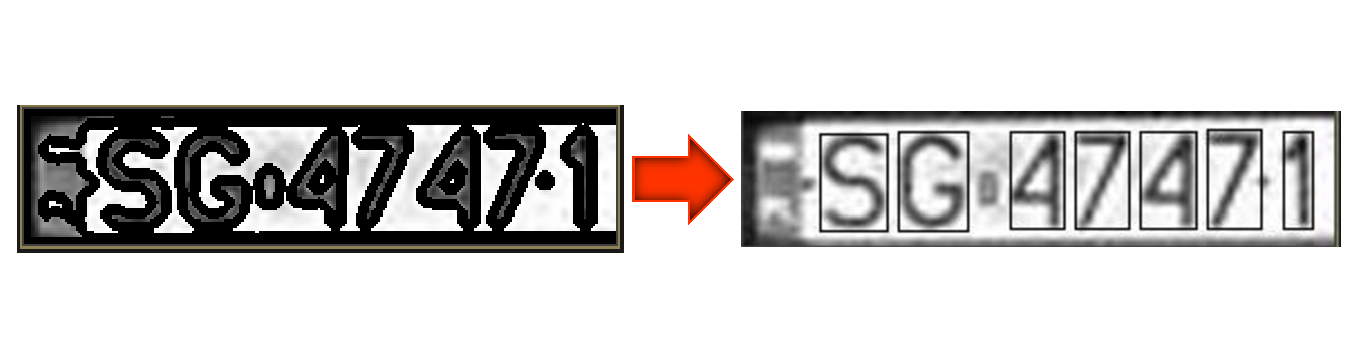
\includegraphics[width=\textwidth]{img/contours}
    \end{center}
\end{frame}

\begin{frame}{Character auslesen und Boundingboxes verschieben}

{\footnotesize Einstellungen für das Auslesen mit Tesseract 5:}
\begin{itemize}
\item {\scriptsize Jeder Character wird einzeln ausgelesen \rightarrow  { }{Page Segmentation Mode(psm10)}}
\item {\scriptsize Engine Mode oem3}
\item {\scriptsize Zeichen-Whitelist (Großbuchstaben + Zahlen 0-9)}
\item {\scriptsize Außerdem: Bild darf nicht zu nahe am Character ausgeschnitten werden (siehe Code)}

\begin{center}
    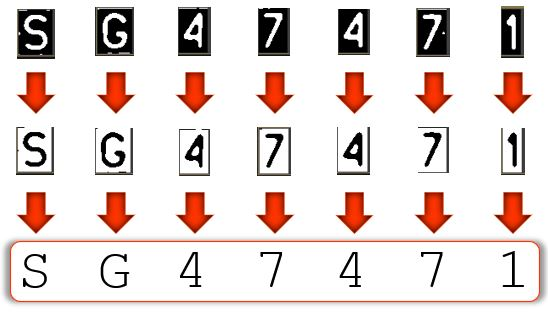
\includegraphics[width=\textwidth,keepaspectratio]{img/char_preprocessing.jpg}
\end{center}

\end{itemize}
\end{frame}


\begin{frame}{Boundingboxes verschieben}
Idee: Falls keine Character in der gefundenen Bounding-Box erkannt werden, verschiebe die Bounding-Box anhand unterschiedlicher Methoden: {\textit hoch, runter, rechts, links, oben-rechts, unten-rechts, unten-links, oben-links}
\begin{center}
    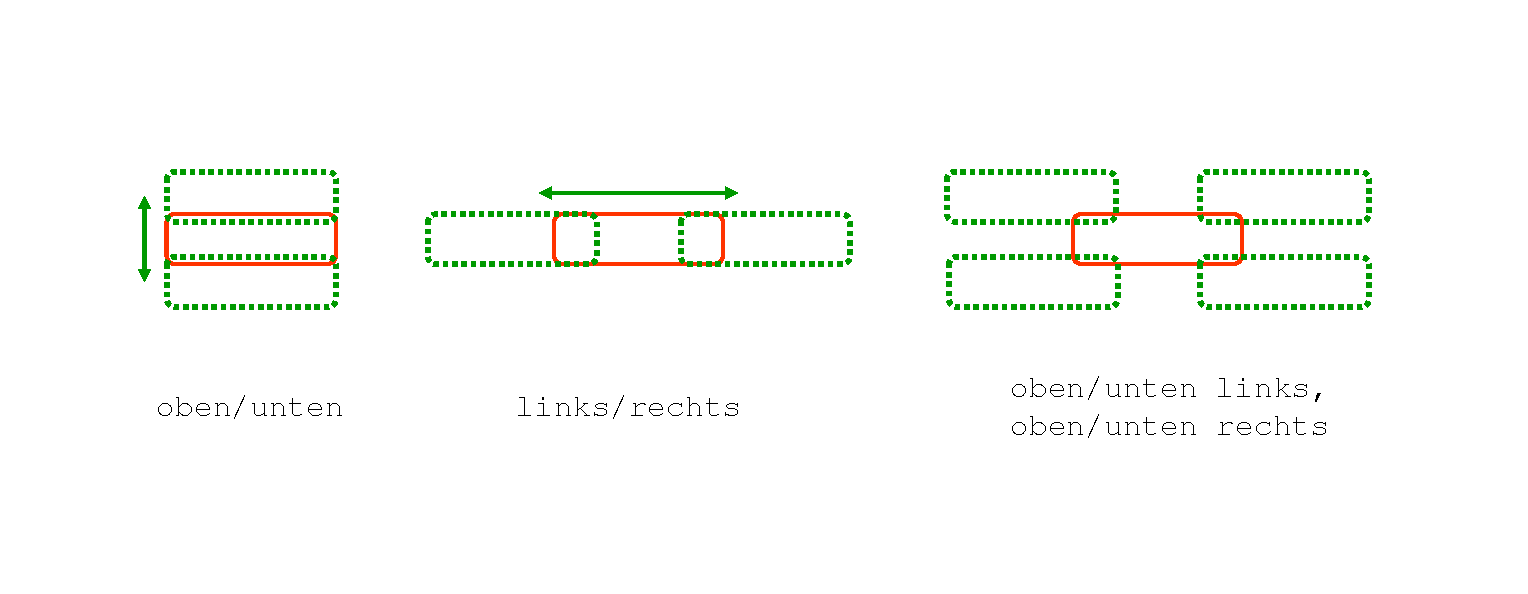
\includegraphics[width=\textwidth]{img/bbox_shift}
\end{center}
\end{frame}
